\documentclass[11pt]{article}

\usepackage[margin=1in]{geometry}
\usepackage{fontspec}
\setmainfont{Bitstream Charter}
\setsansfont{DejaVu Sans}
\setmonofont{DejaVu Sans Mono}
\usepackage[protrusion=false]{microtype}
\usepackage{setspace}
\onehalfspacing
\usepackage{amsmath,amssymb,amsthm,mathtools,bm}
\usepackage{booktabs,tabularx,array,threeparttable,longtable}
\usepackage{graphicx}
\usepackage{subcaption}
\usepackage[dvipsnames]{xcolor}
\usepackage{enumitem}
\usepackage{fancyhdr}
\usepackage{lastpage}
\usepackage[authoryear,round]{natbib}
\usepackage{hyperref}
\usepackage[nameinlink,capitalize,noabbrev]{cleveref}

\definecolor{navy}{HTML}{17365D}
\definecolor{teal}{HTML}{1B7F79}
\definecolor{lightblue}{HTML}{EDF4FA}
\definecolor{lightgray}{HTML}{F4F5F7}
\hypersetup{
  colorlinks=true,
  linkcolor=navy,
  citecolor=teal,
  urlcolor=navy,
  pdftitle={Using Partially Observed Confounder Patterns under Monotone Sequential MAR},
  pdfauthor={Keivan Bolouri Siahkhalehsar}
}

\pagestyle{fancy}
\fancyhf{}
\fancyhead[L]{\small Draft for scientific review}
\fancyhead[R]{\small Pattern-aware causal inference}
\fancyfoot[C]{\small \thepage\ of \pageref*{LastPage}}
\renewcommand{\headrulewidth}{0.4pt}

\newtheorem{assumption}{Assumption}
\newtheorem{theorem}{Theorem}
\newtheorem{proposition}{Proposition}
\newtheorem{corollary}{Corollary}
\newtheorem{lemma}{Lemma}
\theoremstyle{definition}
\newtheorem{remark}{Remark}
\crefname{assumption}{Assumption}{Assumptions}
\Crefname{assumption}{Assumption}{Assumptions}
\crefname{theorem}{Theorem}{Theorems}
\crefname{proposition}{Proposition}{Propositions}
\crefname{corollary}{Corollary}{Corollaries}
\crefname{lemma}{Lemma}{Lemmas}

\newcommand{\E}{\mathbb{E}}
\newcommand{\Pp}{\mathbb{P}}
\newcommand{\Var}{\operatorname{Var}}
\newcommand{\Cov}{\operatorname{Cov}}
\newcommand{\indep}{\perp\!\!\!\perp}
\newcommand{\expit}{\operatorname{expit}}
\newcommand{\norm}[1]{\left\lVert #1\right\rVert_2}
\newcommand{\1}{\mathbbm{1}}
\newcommand{\cc}{\mathrm{cc}}
\newcommand{\seq}{\mathrm{seq}}
\newcommand{\F}{\mathrm{F}}

\title{\vspace{-1.2cm}\textbf{Using Partially Observed Confounder Patterns under Monotone Sequential MAR: Efficient Estimation and the Cost of Complete-Case Coarsening}}
\author{Keivan Bolouri Siahkhalehsar\\
\small Department of Statistics, University of California, Irvine}
\date{September 8, 2026\\[4pt]\small Manuscript draft for scientific review; authorship is provisional}

\begin{document}
\maketitle

\begin{center}
\fcolorbox{navy}{lightblue}{\parbox{0.91\textwidth}{\small
\textbf{Review status.} This document is a research manuscript draft, not a submitted or peer-reviewed article. The theoretical results and software have been internally checked, and the reported primary simulation was independently rerun from the archived code. Independent statistical review, a larger estimated-nuisance simulation, and a substantive data application remain necessary before journal submission.}}
\end{center}

\begin{abstract}
Methods for causal inference with several missing confounders often replace the full missingness pattern by a single indicator that all confounders are observed. This complete-case coarsening is convenient, but it discards records in which some confounders are observed and may require a stronger missingness assumption. We study a binary point exposure and two ordered, partially observed baseline confounders under monotone sequential missing at random (MAR). We specialize the standard sequential coarsening-at-random transformation to the full-data efficient influence function for the average treatment effect (ATE), give a tangent-space proof that the resulting observed-data influence function is canonical, and construct a cross-fitted one-step estimator. An exact drift identity yields sequential multiple robustness. In the common submodel in which both the sequential and complete-case assumptions are valid, we show that the efficiency-bound penalty from complete-case coarsening is
\[
\E\!\left[\frac{1-\pi_2(Z_0)}{\pi_1(Z_0)\pi_2(Z_0)}
\{Q_1(Z_1)-Q_0(Z_0)\}^2\right]\ge 0.
\]
The improvement is strict precisely when the intermediate confounder carries information about the full-data efficient score and second-stage missingness occurs. In an oracle-nuisance experiment with 2,000 samples of size 2,500, retaining the intermediate pattern reduced variance by 4.46\% (paired-bootstrap Monte Carlo 95\% interval, 2.71\%--6.30\%), close to the 4.23\% reduction obtained by numerical evaluation of the identity. When second-stage observation depended on the intermediate confounder, complete-case MAR failed: the coarsened estimator had bias $-0.0322$ and 46.9\% coverage, whereas the sequential estimator had bias $0.0004$ and 95.45\% coverage. The results clarify when partial records improve precision and when coarsening instead changes identification.
\end{abstract}

\noindent\textbf{Keywords:} average treatment effect; efficient influence function; missing confounders; monotone missingness; multiple robustness; sequential MAR.

\section{Introduction}

Observational studies frequently combine two statistical difficulties: treatment is confounded, and one or more baseline confounders are missing. Complete-case analysis is generally inefficient and can be biased. Multiple imputation, inverse-probability weighting, augmented estimators, generalized raking, and targeted learning address parts of this problem, but their validity depends on how the causal and missingness assumptions fit the observed-data structure \citep{bang2005,williamson2012,seaman2014,levis2025,benz2025,williamson2026,wen2026}.

\citet{levis2025} developed robust and efficient ATE estimators under complete-case missing at random (CCMAR). If $L_c$ denotes fully observed confounders, $L_p$ the vector of partially observed confounders, and $S$ the indicator that every component of $L_p$ is observed, their assumption is
\[
S\indep L_p\mid (L_c,A,Y).
\]
The reduction to $S$ avoids modeling a possibly nonmonotone collection of response patterns. It also means that subjects with only part of $L_p$ observed do not directly contribute their observed confounder values to the final estimating function. Levis and colleagues identify the use of such partial records under alternative assumptions as an important direction for future research.

This paper studies the transparent special case in which the components of $L_p$ have a scientifically meaningful order and are observed monotonically. We write
\[
L_c=W,\qquad L_p=(L_1,L_2),
\]
so the notation $L_1,L_2$ refines---rather than replaces---the earlier $L_c,L_p$ notation. The possible patterns are: neither partially observed confounder is available; $L_1$ alone is available; or both are available. Sequential MAR permits the probability of observing $L_2$ to depend on the already observed $L_1$. This model is useful when, for example, an inexpensive screening variable precedes a more burdensome laboratory measure, or when data acquisition follows an ordered protocol.

Sequential inverse-probability augmentation and efficient estimation with monotone missingness are established ideas \citep{rrz1994,gill1997,tsiatis2006,barnwell2025}. Accordingly, our contribution is not the generic sequential augmentation formula. It is the following causal and comparative analysis:
\begin{enumerate}[leftmargin=*,itemsep=3pt]
\item We specialize the monotone sequential construction to the full-data efficient score for a point-exposure ATE with missing confounders, allowing response probabilities to depend on the fully observed treatment and outcome.
\item We give a self-contained observed-likelihood and tangent-space proof of the efficient influence function, followed by an exact remainder identity and a cross-fitted estimator.
\item On the submodel where sequential MAR and CCMAR are simultaneously valid, we derive the exact nonnegative efficiency loss from collapsing the intermediate pattern.
\item We distinguish this efficiency comparison from the case in which second-stage response depends on $L_1$. There, CCMAR generally fails, so the comparison concerns identification, bias, and coverage rather than two efficiency bounds for the same model.
\end{enumerate}

The final distinction is practically important. A statement that the pattern-aware method is ``more efficient'' is justified only under common validity. Outside that submodel, better mean-squared error may result primarily from removing bias under a different, weaker missingness assumption.

\section{Observed data, causal target, and assumptions}

\subsection{Notation and observation patterns}

For one individual, let
\[
Z_0=(W,A,Y),\qquad Z_1=(Z_0,L_1),\qquad Z_2=(Z_1,L_2),
\]
where $W$ is a vector of fully observed baseline confounders, $A\in\{0,1\}$ is a fully observed point exposure, $Y$ is a fully observed outcome, and $L_1,L_2$ are partially observed baseline confounders. Let $R_1$ indicate that $L_1$ is observed. Among records with $R_1=1$, let $C_2$ indicate that $L_2$ is observed, and define $R_2=R_1C_2$. Thus
\[
(R_1,R_2)\in\{(0,0),(1,0),(1,1)\};
\]
the $L_2$-only pattern $(0,1)$ is excluded. The observed datum is
\[
O=(Z_0,R_1,R_1L_1,R_2,R_2L_2).
\]

\begin{table}[ht]
\centering
\caption{Relationship between the original CCMAR notation and the ordered notation used here.}
\label{tab:notation}
\begin{tabularx}{0.92\textwidth}{@{}lXX@{}}
\toprule
Object & CCMAR notation & Sequential notation \\
\midrule
Always observed confounders & $L_c$ & $W$ \\
Partially observed confounders & $L_p$ & $(L_1,L_2)$ \\
Complete-case indicator & $S$ & $R_2=R_1C_2$ \\
Intermediate partial record & discarded by coarsening & $R_1=1,R_2=0$ \\
\bottomrule
\end{tabularx}
\end{table}

Let $V=(W,L_1,L_2)$. The causal estimand is
\[
\psi=\E\{Y(1)-Y(0)\}.
\]

\begin{assumption}[Causal identification]\label{ass:causal}
For $a\in\{0,1\}$: (i) consistency, $Y=Y(A)$; (ii) conditional exchangeability, $Y(a)\indep A\mid V$; and (iii) treatment positivity, $\epsilon<e(V)<1-\epsilon$ almost surely for some $\epsilon>0$, where $e(v)=\Pp(A=1\mid V=v)$.
\end{assumption}

Under \cref{ass:causal}, writing $\mu_a(v)=\E(Y\mid A=a,V=v)$,
\begin{equation}\label{eq:ate-gformula}
\psi=\E\{\mu_1(V)-\mu_0(V)\}.
\end{equation}

\subsection{Sequential missing at random}

\begin{assumption}[Monotone sequential MAR]\label{ass:smar}
The response process satisfies
\begin{align}
R_1&\indep (L_1,L_2)\mid Z_0,\label{eq:mar1}\\
C_2&\indep L_2\mid (Z_1,R_1=1).\label{eq:mar2}
\end{align}
Let
\[
\pi_1(Z_0)=\Pp(R_1=1\mid Z_0),\qquad
\pi_2(Z_1)=\Pp(C_2=1\mid R_1=1,Z_1),
\]
and suppose $\pi_j\ge\epsilon>0$ almost surely for $j=1,2$.
\end{assumption}

Treatment and outcome are included in $Z_0$, so both response probabilities may depend on $A$ and $Y$. These are MAR/CAR restrictions because the hazards depend only on information observed at the corresponding stage. They are not outcome-independent missing-not-at-random restrictions.

\begin{proposition}[Identification of the full-data law]\label{prop:identification}
Under \cref{ass:smar}, the full-data density is identified by
\begin{equation}\label{eq:full-law-identification}
p(z_0,l_1,l_2)
=p(z_0)\,p(l_1\mid z_0,R_1=1)\,
p(l_2\mid z_1,R_1=1,C_2=1).
\end{equation}
Consequently, under \cref{ass:causal}, $\psi$ in \cref{eq:ate-gformula} is identified from the observed-data law.
\end{proposition}

\begin{proof}
By \cref{eq:mar1}, $p(l_1,l_2\mid z_0,R_1=1)=p(l_1,l_2\mid z_0)$, hence $p(l_1\mid z_0,R_1=1)=p(l_1\mid z_0)$. By \cref{eq:mar2}, among $R_1=1$, $p(l_2\mid z_1,C_2=1)=p(l_2\mid z_1)$. Combining these conditional densities with $p(z_0)$ gives \cref{eq:full-law-identification}. The g-formula is a functional of the identified full-data law.
\end{proof}

Equation \cref{eq:full-law-identification} is a retrospective factorization because $A$ and $Y$ occur in $Z_0$. This causes no contradiction with the causal factorization: any identified joint law can also be refactored as $p(v)p(a\mid v)p(y\mid a,v)$, after which \cref{ass:causal} gives the causal interpretation.

\section{Efficient influence function under sequential MAR}

\subsection{Full-data gradient}

The efficient influence function for the ATE in the nonparametric full-data model is
\begin{equation}\label{eq:full-eif}
D_{\F}(Z_2)=G(Z_2)-\psi,
\end{equation}
where
\begin{equation}\label{eq:G}
G(Z_2)=\mu_1(V)-\mu_0(V)
+\frac{A}{e(V)}\{Y-\mu_1(V)\}
-\frac{1-A}{1-e(V)}\{Y-\mu_0(V)\}.
\end{equation}
Define the iterated projections
\begin{equation}\label{eq:Qs}
Q_1(Z_1)=\E\{G(Z_2)\mid Z_1\},\qquad
Q_0(Z_0)=\E\{G(Z_2)\mid Z_0\}.
\end{equation}

\begin{theorem}[Canonical gradient]\label{thm:eif}
Suppose \cref{ass:causal,ass:smar} hold and $D_{\F}\in L_2(P)$. In the nonparametric observed-data model induced by monotone sequential MAR, the efficient influence function for $\psi$ is
\begin{equation}\label{eq:seq-eif}
\boxed{
D_{\seq}(O)=Q_0-\psi
+\frac{R_1}{\pi_1}(Q_1-Q_0)
+\frac{R_2}{\pi_1\pi_2}(G-Q_1).}
\end{equation}
All functions in a term are evaluated only when the variables required for that term are observed.
\end{theorem}

\begin{proof}
We give the observed-likelihood argument. Write
\[
p_0(z_0)=p(z_0),\quad p_1(l_1\mid z_0)=p(l_1\mid z_0),\quad
p_2(l_2\mid z_1)=p(l_2\mid z_1).
\]
Under \cref{ass:smar}, the observed-data likelihood contribution factorizes as
\begin{align}
p_O(o)
={}&p_0(z_0)
\{1-\pi_1(z_0)\}^{1-r_1}
\{\pi_1(z_0)p_1(l_1\mid z_0)\}^{r_1}\notag\\
&\times\{1-\pi_2(z_1)\}^{r_1-r_2}
\{\pi_2(z_1)p_2(l_2\mid z_1)\}^{r_2}.
\label{eq:observed-likelihood}
\end{align}
For regular parametric submodels, the tangent space is the closure of sums of the mutually orthogonal components
\begin{align*}
\mathcal T_0&=\{s_0(Z_0):\E(s_0)=0\},\\
\mathcal T_1&=\{R_1s_1(Z_1):\E(s_1\mid Z_0)=0\},\\
\mathcal T_2&=\{R_2s_2(Z_2):\E(s_2\mid Z_1)=0\},\\
\mathcal T_{\pi_1}&=\{(R_1-\pi_1)h_1(Z_0)\},\\
\mathcal T_{\pi_2}&=\{(R_2-R_1\pi_2)h_2(Z_1)\}.
\end{align*}
Let $q_1=\E(D_{\F}\mid Z_1)=Q_1-\psi$ and
$q_0=\E(D_{\F}\mid Z_0)=Q_0-\psi$. Candidate \cref{eq:seq-eif} can be written
\begin{equation}\label{eq:eif-centered}
D_{\seq}=q_0+\frac{R_1}{\pi_1}(q_1-q_0)
+\frac{R_2}{\pi_1\pi_2}(D_{\F}-q_1).
\end{equation}
The three terms in \cref{eq:eif-centered} belong respectively to
$\mathcal T_0,\mathcal T_1,$ and $\mathcal T_2$: the required conditional means vanish by iterated expectation. Thus $D_{\seq}$ belongs to the observed-data tangent space and is orthogonal to the two response-mechanism tangent components.

It remains to verify that $D_{\seq}$ represents the pathwise derivative. For $s_0\in\mathcal T_0$,
\[
\E(D_{\seq}s_0)=\E(q_0s_0)=\E(D_{\F}s_0).
\]
For a full-law score $s_1$ satisfying $\E(s_1\mid Z_0)=0$, the observed score is $R_1s_1$, and conditional expectation over $R_1,C_2$ gives
\[
\E(D_{\seq}R_1s_1)=\E\{(q_1-q_0)s_1\}=\E(D_{\F}s_1).
\]
The last equality uses $\E(s_1\mid Z_0)=0$ and $q_1=\E(D_{\F}\mid Z_1)$. Similarly, for $s_2$ satisfying $\E(s_2\mid Z_1)=0$, the observed score is $R_2s_2$ and
\[
\E(D_{\seq}R_2s_2)=\E\{(D_{\F}-q_1)s_2\}=\E(D_{\F}s_2).
\]
Finally, $\psi$ does not depend on $\pi_1$ or $\pi_2$, and the inner products of $D_{\seq}$ with their score components are zero. Hence \cref{eq:eif-centered} represents the derivative along every tangent direction. Because it lies in the tangent space, it is the canonical gradient and has minimum variance among regular influence functions \citep{tsiatis2006}.
\end{proof}

\begin{remark}
The proof is a two-stage specialization of general monotone-MAR/CAR theory \citep{rrz1994,gill1997,barnwell2025}. Its purpose is to establish rigorously that the causal pseudo-outcome in \cref{eq:G}, after sequential projection, yields the efficient observed-data gradient for this particular ATE problem.
\end{remark}

\section{Estimation, robustness, and inference}

\subsection{Cross-fitted one-step estimator}

Let $\eta=(e,\mu_0,\mu_1,\pi_1,\pi_2,Q_0,Q_1)$. With nuisance estimates trained outside observation $i$'s validation fold, define
\begin{equation}\label{eq:Hhat}
\widehat H_i=widehat Q_{0,i}
+\frac{R_{1i}}{\widehat\pi_{1,i}}(\widehat Q_{1,i}-\widehat Q_{0,i})
+\frac{R_{2i}}{\widehat\pi_{1,i}\widehat\pi_{2,i}}
(\widehat G_i-\widehat Q_{1,i}),
\end{equation}
and
\begin{equation}\label{eq:estimator}
\widehat\psi_{\seq}=\frac{1}{n}\sum_{i=1}^n\widehat H_i.
\end{equation}
An estimated standard error is
\begin{equation}\label{eq:se}
\widehat{\mathrm{se}}(\widehat\psi_{\seq})
=\left[\frac{1}{n(n-1)}\sum_{i=1}^n
(\widehat H_i-\widehat\psi_{\seq})^2\right]^{1/2}.
\end{equation}

One practical training sequence is: fit $\pi_1$ to all training records; fit $\pi_2$ among $R_1=1$ records; fit the causal regressions on complete records with inverse-response weights to reconstruct the full law; regress $\widehat G$ on $Z_1$ among complete records to obtain $Q_1$; and regress the stage-two augmented pseudo-outcome on $Z_0$ among $R_1=1$ records to obtain $Q_0$. Other learners are possible, provided they estimate the same nuisance functions and the positivity and convergence conditions below are respected.

\subsection{Exact drift and sequential multiple robustness}

For arbitrary fixed functions $\bar G,\bar Q_0,\bar Q_1,\bar\pi_1,\bar\pi_2$, define
\[
Q_1^{\bar G}=\E(\bar G\mid Z_1),\qquad
Q_0^{\bar G}=\E(\bar G\mid Z_0),
\]
and let $H(\bar\eta)$ denote \cref{eq:Hhat} with bars in place of hats.

\begin{proposition}[Exact missingness-layer drift]\label{prop:drift}
Under \cref{ass:smar},
\begin{align}
\E\{H(\bar\eta)\}-\E(\bar G)
={}&\E\!\left[\left(1-\frac{\pi_1}{\bar\pi_1}\right)
(\bar Q_0-Q_0^{\bar G})\right]\notag\\
&+\E\!\left[\frac{\pi_1}{\bar\pi_1}
\left(1-\frac{\pi_2}{\bar\pi_2}\right)
(\bar Q_1-Q_1^{\bar G})\right].
\label{eq:missing-drift}
\end{align}
If $\bar G$ is formed from $(\bar e,\bar\mu_0,\bar\mu_1)$ as in \cref{eq:G}, then
\begin{align}
\E(\bar G)-\psi
=\E\!\left[
\frac{\bar e-e}{\bar e}(\bar\mu_1-\mu_1)
+\frac{\bar e-e}{1-\bar e}(\bar\mu_0-\mu_0)
\right].
\label{eq:causal-drift}
\end{align}
\end{proposition}

\begin{proof}
Taking expectation of $H(\bar\eta)$ over the response indicators conditional on the full data replaces $R_1$ by $\pi_1$ and $R_2$ by $\pi_1\pi_2$. Subtracting $\E(\bar G)$ and adding and subtracting $Q_j^{\bar G}$ yields \cref{eq:missing-drift}; the terms involving $Q_j^{\bar G}$ reduce to conditional expectations of $\bar G$. For \cref{eq:causal-drift}, condition the barred version of \cref{eq:G} on $V$, use $\E(A\mid V)=e(V)$ and $\E(Y\mid A=a,V)=\mu_a(V)$, then collect products of the treatment- and outcome-regression errors.
\end{proof}

\begin{corollary}[Sequential multiple robustness]\label{cor:robustness}
The estimating equation is unbiased for $\psi$ under every nuisance configuration satisfying all three clauses:
\begin{enumerate}[label=(\roman*),leftmargin=*]
\item $\bar e=e$ or $(\bar\mu_0,\bar\mu_1)=(\mu_0,\mu_1)$;
\item $\bar\pi_1=\pi_1$ or $\bar Q_0=Q_0^{\bar G}$;
\item $\bar\pi_2=\pi_2$ or $\bar Q_1=Q_1^{\bar G}$.
\end{enumerate}
This gives up to $2\times2\times2=8$ sufficient configurations. The result is a layered or sequential form of multiple robustness, not a claim that any arbitrary subset of nuisance models may be misspecified.
\end{corollary}

\subsection{Asymptotic normality}

\begin{theorem}[Cross-fitted asymptotic linearity]\label{thm:asymptotics}
Use a fixed number of folds. Suppose, uniformly across folds: (i) fitted observation probabilities and treatment probabilities are bounded away from zero (and the treatment probability from one); (ii) $\norm{\widehat H-H(\eta)}=o_p(1)$ and the influence functions have uniformly integrable $2+\delta$ moments for some $\delta>0$; and (iii)
\begin{align*}
&\norm{\widehat e-e}
\{\norm{\widehat\mu_1-\mu_1}+\norm{\widehat\mu_0-\mu_0}\}
=o_p(n^{-1/2}),\\
&\norm{\widehat\pi_1-\pi_1}\,
\norm{\widehat Q_0-Q_0^{\widehat G}}=o_p(n^{-1/2}),\\
&\norm{\widehat\pi_2-\pi_2}\,
\norm{\widehat Q_1-Q_1^{\widehat G}}=o_p(n^{-1/2}).
\end{align*}
Then
\[
\sqrt n(\widehat\psi_{\seq}-\psi)
=\frac{1}{\sqrt n}\sum_{i=1}^nD_{\seq}(O_i)+o_p(1)
\rightsquigarrow N\{0,\Var(D_{\seq})\}.
\]
The variance estimator in \cref{eq:se} is consistent, and the estimator attains the semiparametric efficiency bound.
\end{theorem}

\begin{proof}
Conditional on the training samples, cross-fitting makes each validation-fold nuisance fit fixed. Decompose $\widehat\psi-\psi$ into the empirical mean of the true influence function, an empirical-process difference on the validation fold, and the conditional drift. The $L_2$ convergence in (ii) makes the second term $o_p(n^{-1/2})$ without Donsker conditions. Applying \cref{prop:drift} fold by fold and Cauchy--Schwarz bounds the drift by the three products in (iii), up to constants from positivity. Thus the remainder is $o_p(n^{-1/2})$. The central limit theorem applies to the first term. Consistency of the empirical second moment follows from (ii) and uniform integrability. Efficiency follows from \cref{thm:eif}. This is the standard cross-fitting argument \citep{chernozhukov2018} specialized to \cref{eq:seq-eif}.
\end{proof}

The conditions do not require every nuisance to converge at $n^{-1/4}$; that rate for each member of a product is merely a simple sufficient condition. Very small response probabilities remain a practical threat even when formal positivity holds, motivating weight diagnostics, truncation sensitivity analyses, and estimators targeted for finite-sample stability.

\section{Exact cost of complete-case coarsening}

Let $S=R_2$ and suppose the analyst replaces $(R_1,R_2)$ by the single complete-case indicator $S$. The next restriction creates a submodel in which both approaches identify the same target.

\begin{assumption}[Common-validity submodel]\label{ass:common}
The second-stage response probability does not depend on the intermediate confounder after $Z_0$:
\[
\pi_2(Z_1)=\pi_2(Z_0).
\]
\end{assumption}

Then $S\indep(L_1,L_2)\mid Z_0$, with $\Pp(S=1\mid Z_0)=\pi_1(Z_0)\pi_2(Z_0)$, so CCMAR holds. The efficient influence function based only on
$O^{\cc}=(Z_0,S,SL_1,SL_2)$ is
\begin{equation}\label{eq:cc-eif}
D_{\cc}(O^{\cc})=Q_0-\psi+
\frac{S}{\pi_1\pi_2}(G-Q_0).
\end{equation}

\begin{theorem}[Efficiency loss from collapsing the pattern]\label{thm:gap}
Under \cref{ass:causal,ass:smar,ass:common},
\begin{equation}\label{eq:difference}
D_{\cc}-D_{\seq}
=\frac{R_1}{\pi_1}\left(\frac{C_2}{\pi_2}-1\right)(Q_1-Q_0),
\end{equation}
and this difference is orthogonal to $D_{\seq}$. Consequently,
\begin{equation}\label{eq:variance-gap}
\boxed{
\Var(D_{\cc})-\Var(D_{\seq})
=\E\!\left[
\frac{1-\pi_2(Z_0)}{\pi_1(Z_0)\pi_2(Z_0)}
\{Q_1(Z_1)-Q_0(Z_0)\}^2
\right]\ge0.}
\end{equation}
\end{theorem}

\begin{proof}
Expanding \cref{eq:cc-eif} and subtracting \cref{eq:seq-eif} gives \cref{eq:difference}. Let $\Delta=Q_1-Q_0$ and $\varepsilon=G-Q_1$. Conditional on $Z_1$, $\E(\varepsilon\mid Z_1)=0$; conditional on $Z_1,R_1=1$, $\E(C_2/\pi_2-1)=0$. Multiplying \cref{eq:difference} by the three orthogonal increments in \cref{eq:seq-eif} and applying these conditional-mean properties shows
$\E\{(D_{\cc}-D_{\seq})D_{\seq}\}=0$. Finally,
\begin{align*}
\E\{(D_{\cc}-D_{\seq})^2\mid Z_1\}
&=\frac{1-\pi_2(Z_0)}{\pi_1(Z_0)\pi_2(Z_0)}\Delta^2,
\end{align*}
because $R_1$ and $C_2$ are Bernoulli with the stated sequential probabilities. Pythagoras gives \cref{eq:variance-gap}.
\end{proof}

\begin{corollary}[When the gain is strict]\label{cor:strict}
The pattern-aware efficiency bound is strictly smaller if and only if
\[
\Pp\!\left[pi_2(Z_0)<1\ \text{and}\ Q_1(Z_1)\ne Q_0(Z_0)\right]>0.
\]
Equivalently, strict improvement requires second-stage missingness and residual predictive information in $L_1$ about the full-data efficient score after conditioning on $Z_0$.
\end{corollary}

When $\pi_2$ depends on $L_1$, the complete-case probability conditional on $Z_0$ averages over an unobserved determinant of selection, and $S\indep(L_1,L_2)\mid Z_0$ generally fails. Then \cref{eq:variance-gap} is not an efficiency comparison: the coarsened estimator may target the wrong observed-data functional. This is the distinction between an \emph{information loss} under common validity and an \emph{identification failure} under sequential MAR alone.

\section{Simulation studies}

\subsection{Design}

The primary experiment isolates the missingness layer by using oracle nuisance functions. It contains $2{,}000$ independently generated samples of size $n=2{,}500$ under each of two response mechanisms, with random seed 20260831. No $W$ variables are included. The joint full-data law is specified retrospectively:
\begin{align*}
A&\sim\mathrm{Bernoulli}(0.5),\\
Y\mid A=0&\sim\mathrm{Beta}(2,4),\qquad
Y\mid A=1\sim\mathrm{Beta}(4,2),\\
L_1\mid A,Y&\sim\mathrm{Bernoulli}\{\expit(-0.6+0.5A+0.25Y+0.1AY)\},\\
L_2\mid A,Y,L_1&\sim N(A+Y+2.5L_1Y,1.25^2).
\end{align*}
Numerical refactorization of this joint law gives $e(V)$ and $\mu_a(V)$; numerical integration gives the true ATE $\psi=0.2558486$. Response at stage one follows
\[
\pi_1=\expit(2+0.1A+0.1Y).
\]
In the CCMAR-compatible scenario,
\[
\pi_2=\expit(-1.1+0.1A+0.1Y),
\]
whereas in the sequential-MAR scenario,
\[
\pi_2=\expit(-1.9+0.1A+0.1Y+2.2L_1).
\]
The first permits an efficiency comparison; the second violates CCMAR and permits an identification comparison. Confidence intervals use the empirical variance of the oracle influence values in each sample.

Three estimators are reported: the full-data ATE estimator, the coarsened CCMAR estimator in \cref{eq:cc-eif}, and the pattern-aware sequential estimator in \cref{eq:seq-eif}. A paired bootstrap over the same Monte Carlo replicates quantifies simulation uncertainty in the variance reduction. Separately, the expectation in \cref{eq:variance-gap} was evaluated using $1.5$ million numerical integration draws.

\subsection{Primary results}

\begin{table}[ht]
\centering
\begin{threeparttable}
\caption{Primary oracle-nuisance simulation ($n=2{,}500$, 2,000 replicates).}
\label{tab:main-results}
\small
\begin{tabular}{@{}llrrrr@{}}
\toprule
Scenario & Estimator & Bias & Empirical SD & RMSE & 95\% coverage \\
\midrule
CCMAR-compatible & Full data & $-0.00029$ & 0.01087 & 0.01087 & 94.40\% \\
 & Coarsened CCMAR & $-0.00049$ & 0.01817 & 0.01817 & 94.05\% \\
 & Sequential patterns & $-0.00047$ & 0.01776 & 0.01776 & 94.55\% \\
\addlinespace
Sequential-MAR & Full data & 0.00043 & 0.01038 & 0.01038 & 95.50\% \\
 & Coarsened CCMAR & $-0.03222$ & 0.01831 & 0.03706 & 46.90\% \\
 & Sequential patterns & 0.00044 & 0.01596 & 0.01597 & 95.45\% \\
\bottomrule
\end{tabular}
\begin{tablenotes}[flushleft]\footnotesize
\item Monte Carlo standard errors for bias ranged from 0.00023 to 0.00041; those for coverage ranged from 0.46 to 1.12 percentage points. The target ATE was 0.2558486.
\end{tablenotes}
\end{threeparttable}
\end{table}

The empirical variance ratio (coarsened divided by sequential) was 1.0467 in the common-validity scenario, corresponding to 4.46\% lower variance for the sequential estimator. A paired bootstrap with 10,000 resamples gave a Monte Carlo 95\% interval of 2.71\%--6.30\%. Numerical evaluation of \cref{eq:variance-gap} produced influence-function variances 0.77466 and 0.74193 for the coarsened and sequential methods, respectively: a ratio of 1.0441 and a 4.23\% reduction. The agreement supports the algebraic identity and the simulation implementation.

In the sequential-only scenario, the coarsened estimator's bias was large relative to its standard deviation, and nominal coverage fell to 46.9\%. The sequential estimator remained approximately unbiased with 95.45\% coverage. This contrast should not be described as an efficiency gain, because CCMAR is false in this scenario.

\begin{figure}[ht]
\centering
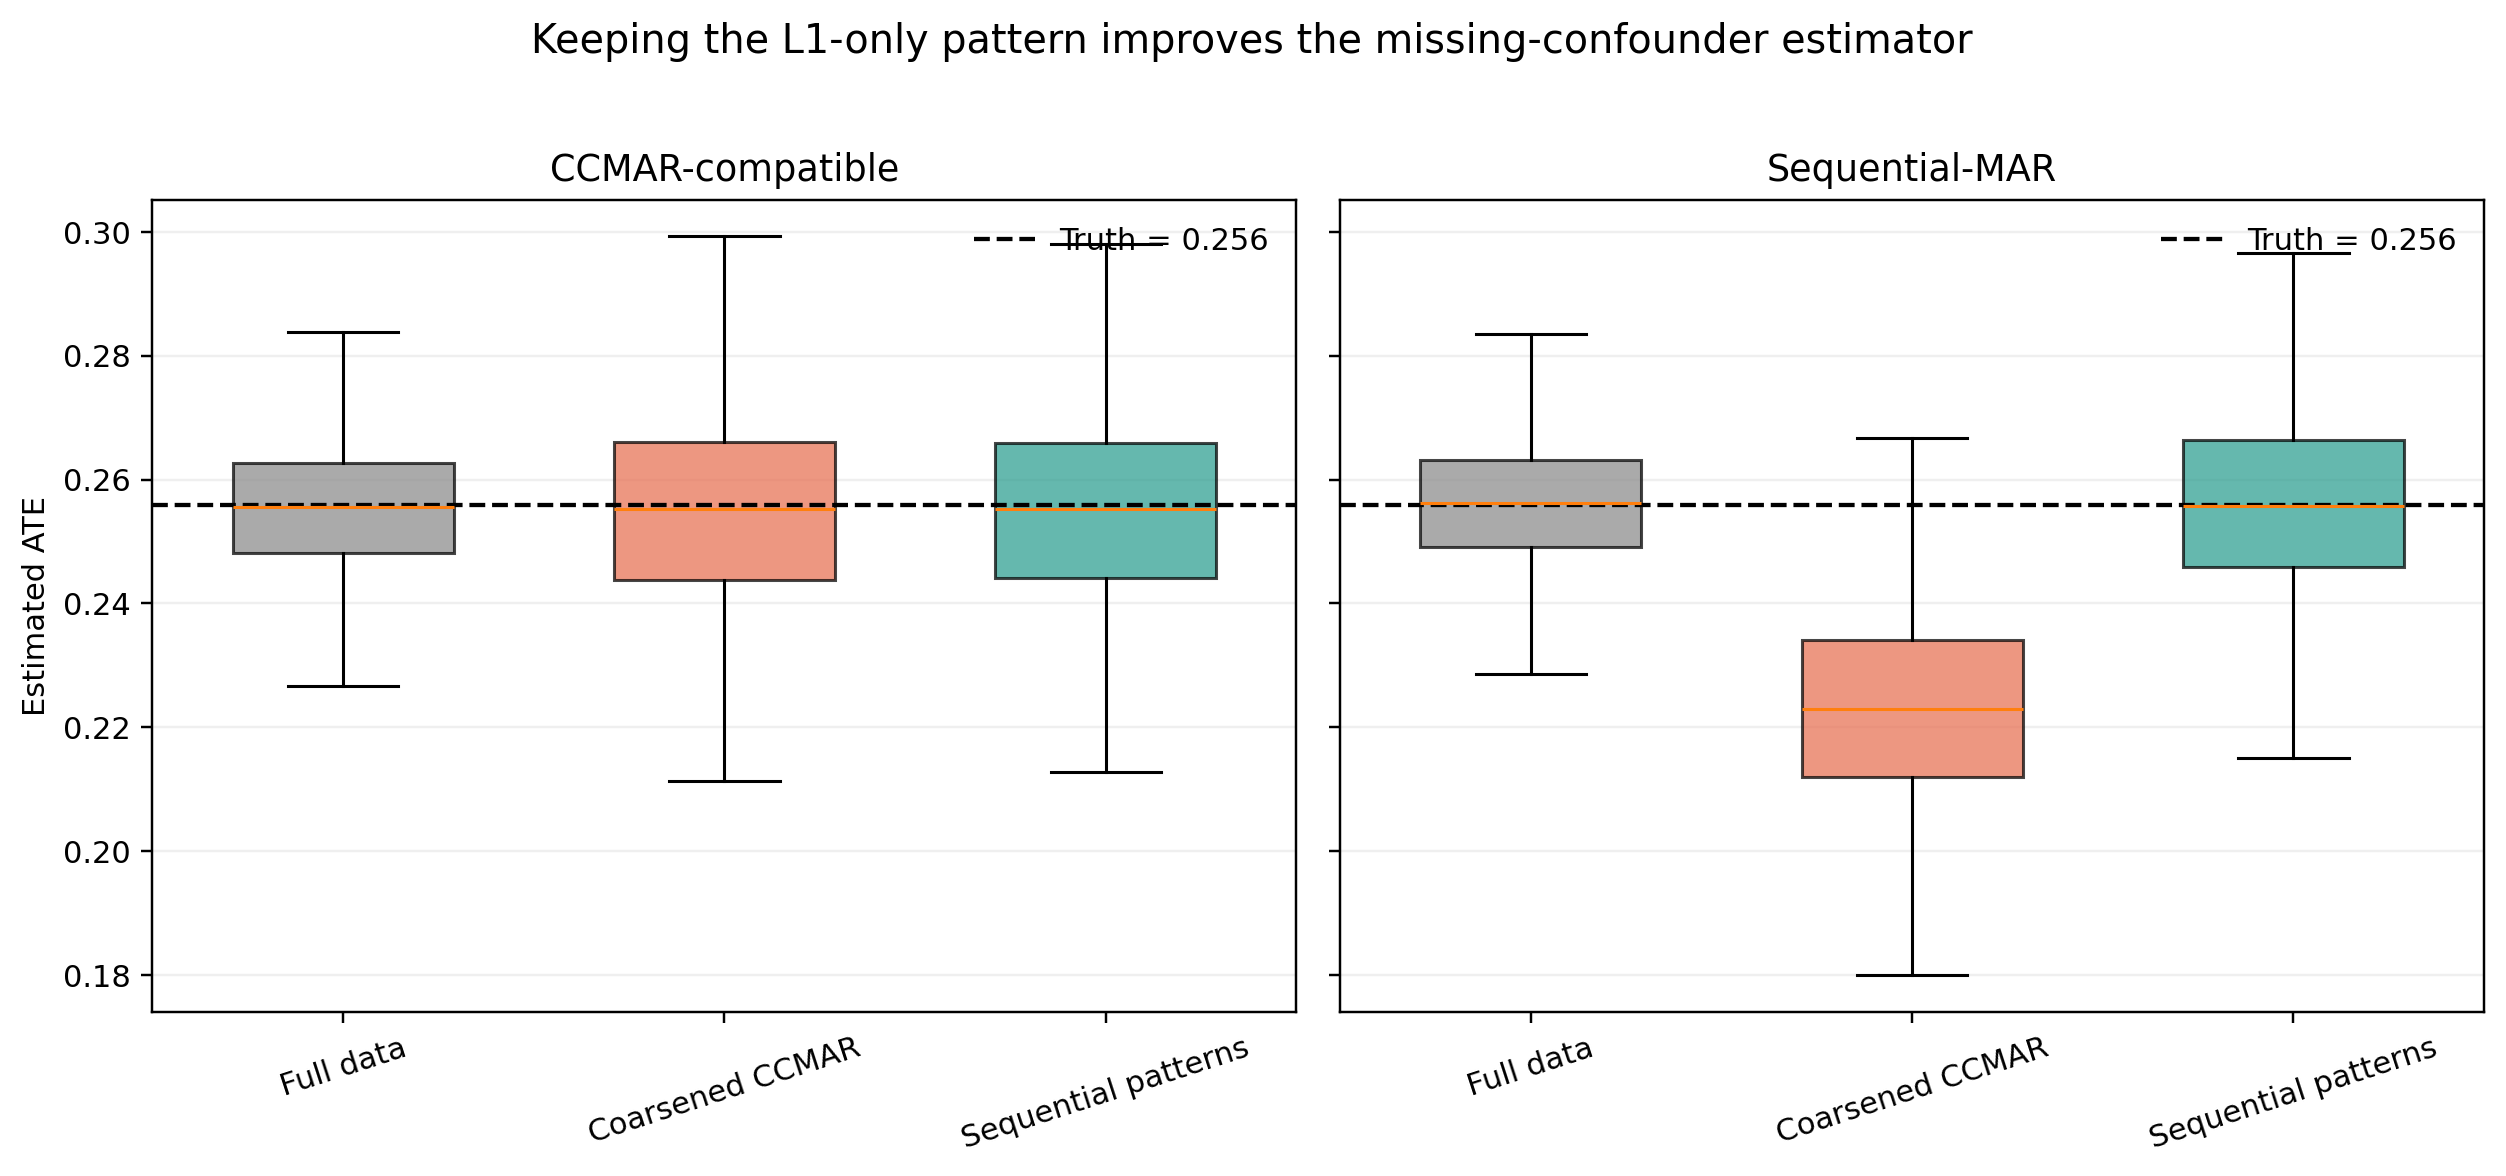
\includegraphics[width=\textwidth]{figures/estimator_comparison.png}
\caption{Distributions of oracle estimates across 2,000 replicates. Boxes show the interquartile range and whiskers extend to the conventional $1.5\times$ interquartile range. The dashed line is the true ATE. The CCMAR-compatible panel compares precision; the sequential-MAR panel primarily displays coarsening bias.}
\label{fig:main-boxplot}
\end{figure}

The mean pattern proportions were 23.98\% complete, 65.09\% $L_1$-only, and 10.93\% neither under common validity; the corresponding values were 31.18\%, 57.89\%, and 10.93\% under sequential MAR.

\subsection{Sensitivity analysis}

A second oracle experiment used 5,000 replicates per condition. Under common validity, the stage-two intercept was varied to change how many records retained only $L_1$. The sequential variance reduction increased from 2.05\% with 51.17\% complete records to 5.53\% with 11.61\% complete records (\cref{tab:sensitivity-efficiency}).

\begin{table}[ht]
\centering
\caption{Efficiency sensitivity under CCMAR (5,000 replicates per row).}
\label{tab:sensitivity-efficiency}
\small
\begin{tabular}{@{}lrrr@{}}
\toprule
Second-stage missingness & Complete & $L_1$ only & Sequential variance reduction \\
\midrule
Low & 51.17\% & 37.90\% & 2.05\% \\
Moderate & 24.00\% & 65.06\% & 3.92\% \\
High & 11.61\% & 77.46\% & 5.53\% \\
\bottomrule
\end{tabular}
\end{table}

In a separate sequence, intercepts were calibrated to keep the complete-case proportion near 24\% while increasing the coefficient $\gamma$ of $L_1$ in the second-stage response logit. Coarsened bias and undercoverage worsened monotonically, while sequential bias remained negligible (\cref{tab:sensitivity-identification}).

\begin{table}[ht]
\centering
\caption{Identification sensitivity as CCMAR departure increases (5,000 replicates per row).}
\label{tab:sensitivity-identification}
\small
\begin{tabular}{@{}rrrrr@{}}
\toprule
$\gamma$ & Coarsened bias & Coarsened coverage & Sequential bias & Sequential coverage \\
\midrule
0.75 & $-0.01415$ & 83.30\% & $-0.00014$ & 95.12\% \\
1.50 & $-0.02657$ & 61.80\% & 0.00011 & 95.12\% \\
2.25 & $-0.03627$ & 45.74\% & 0.00011 & 95.28\% \\
\bottomrule
\end{tabular}
\end{table}

\begin{figure}[ht]
\centering
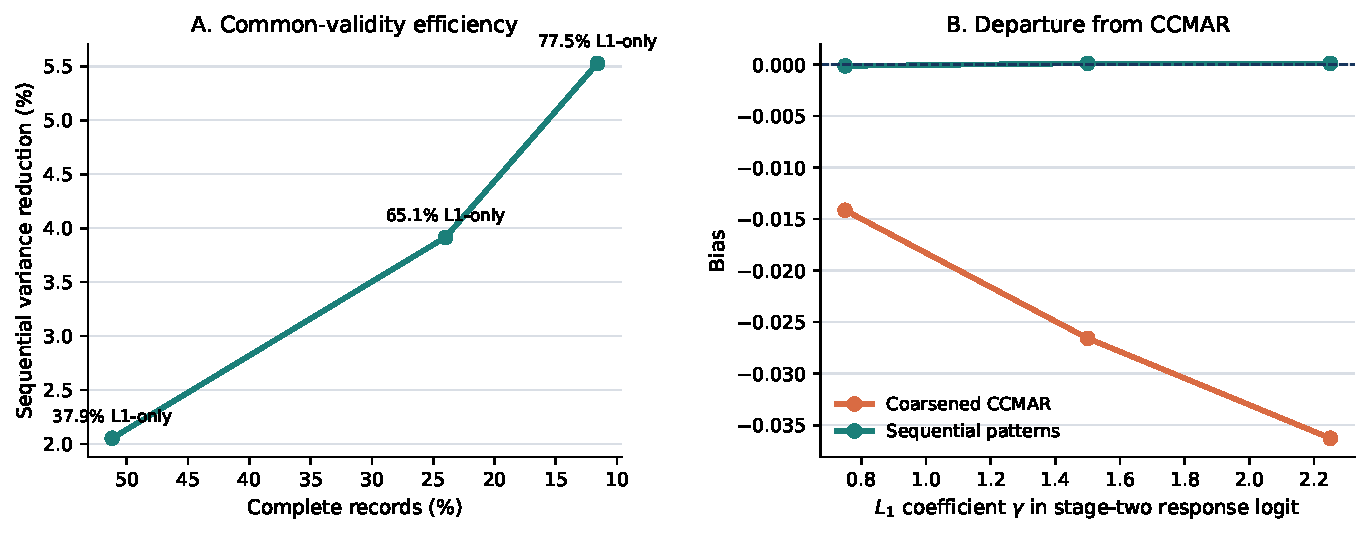
\includegraphics[width=0.96\textwidth]{figures/sensitivity_summary.pdf}
\caption{Sensitivity results. Left: efficiency gain under common validity as complete records become rarer. Right: estimator bias as dependence of second-stage response on $L_1$ increases while the complete-case proportion is held near 24\%.}
\label{fig:sensitivity}
\end{figure}

\subsection{Estimated-nuisance implementation check}

The reproducibility package also contains a fully out-of-fold implementation using weighted treatment and outcome regressions and flexible sequential regressions. In a preliminary 100-replicate check with $n=4{,}000$ and true ATE 0.5, sequential-estimator bias was 0.0068 (Monte Carlo standard error 0.0068) under CCMAR and $-0.0027$ (0.0068) under sequential MAR. Coverage was 91\% and 94\%, respectively. These results confirm that the end-to-end code runs, but 100 replicates are insufficient for precise evaluation, and the 91\% coverage signals that standard-error calibration or nuisance learning may need improvement. We therefore treat this as an implementation check rather than confirmatory evidence.

\section{Discussion}

The exact variance identity gives a direct interpretation of partial-record value. The gain is large when three ingredients coincide: many subjects reach stage one but not stage two; stage-two positivity is not too weak; and $L_1$ predicts the complete-data efficient score beyond $Z_0$. Merely having many $L_1$-only records is not sufficient if $Q_1=Q_0$; conversely, an extremely informative $L_1$ can be of little practical help if almost everyone also has $L_2$.

The model comparison also clarifies assumption strength. Under \cref{ass:common}, complete-case coarsening wastes information but remains valid. If $L_1$ affects the chance that $L_2$ is observed, sequential MAR may remain plausible because that chance depends on information observed at stage two, whereas CCMAR generally fails after $L_1$ is hidden inside the all-complete indicator. In that setting, the pattern-aware estimator is not simply a more precise version of the CCMAR estimator; it is based on a different identifying model.

The present results sit between two literatures. General sequential augmentation and efficiency under monotone attrition are well established \citep{rrz1994,gill1997,barnwell2025}. Recent causal work addresses complete-case MAR \citep{levis2025}, multiple missing confounders or exposures under other MAR/MNAR restrictions \citep{wen2026}, and broad numerical comparisons of practical missing-confounder estimators \citep{benz2025,williamson2026}. The narrow value added here is the exact causal score comparison between retaining and collapsing a monotone intermediate pattern. We do not solve the nonmonotone $2^q$-pattern projection problem under the original CCMAR model, and we do not claim the generic monotone-MAR influence-function transformation as new.

Several limitations delimit the current evidence. First, all numerical results are synthetic; there is no substantive data application. Second, the main and sensitivity simulations use oracle nuisance functions to isolate the missingness mechanism. Third, the estimated-nuisance study is preliminary and does not yet evaluate a broad library of learners, nuisance misspecification configurations, near-positivity, sample sizes, or confidence-interval corrections. Fourth, monotonicity rules out $L_2$-only records and may be implausible in unstructured electronic health records. Fifth, MAR and causal exchangeability are not testable from the observed data alone. Finally, independent expert checking of the canonical-gradient and remainder proofs is necessary before submission.

Before journal submission, the following additions are priorities: (i) a preregistered, larger cross-fitted simulation with at least 1,000--2,000 replicates per design point; (ii) explicit nuisance misspecification and learner comparisons; (iii) weight-truncation and near-positivity sensitivity analyses; (iv) a real or high-fidelity plasmode application with a scientifically defensible ordering of confounder acquisition; (v) a public software interface with unit tests and documented diagnostics; and (vi) independent semiparametric review. Subject to those additions, the paper is best positioned as a focused methods contribution on the cost of complete-case coarsening rather than as a general solution to arbitrary nonmonotone missing confounders.

\section*{Data and code availability}

All data analyzed in this manuscript are synthetic. The accompanying reproducibility package contains the Python programs, random seeds, replicate-level CSV files, numerical variance check, generated figures, and the manuscript source. The primary experiment can be reproduced with
\begin{verbatim}
python code/validate_sequential_mar.py --n 2500 --reps 2000 \
  --seed 20260831 --outdir results/main_verified
\end{verbatim}
The original CCMAR implementation of \citet{levis2025} is available at
\url{https://github.com/alexlevis/flex-ate-confounders-MAR}. That repository is cited as prior software and is not represented as the source of the new sequential-pattern code.

\section*{Reproducibility audit}

The primary Python simulation, summary bootstrap, and numerical variance identity were rerun in a clean working directory. The regenerated truth, replicate, summary, pattern-proportion, bootstrap-summary, and variance-identity files were byte-identical to the archived outputs. The sensitivity and estimated-nuisance summaries were recomputed from their replicate-level files and matched numerically. A smoke test of the cross-fitted implementation completed successfully. The supplied R mirror was not rerun because R was unavailable in the audit environment; Python outputs are therefore the authoritative results for this manuscript.

\section*{Acknowledgments}

This draft was developed for scientific review. Individuals who contribute substantially to conception, derivation, software, interpretation, or revision should be considered for authorship only after explicit discussion and agreement. No additional author is assigned in this draft.

\section*{Funding and conflicts of interest}

To be completed by the author before submission.

\begin{thebibliography}{99}

\bibitem[Bang and Robins(2005)]{bang2005}
Bang, H. and Robins, J. M. (2005).
Doubly robust estimation in missing data and causal inference models.
\emph{Biometrics}, 61(4), 962--973.
\href{https://doi.org/10.1111/j.1541-0420.2005.00377.x}{doi:10.1111/j.1541-0420.2005.00377.x}.

\bibitem[Barnwell and Chaudhuri(2025)]{barnwell2025}
Barnwell, J.-L. and Chaudhuri, S. (2025).
Efficiency in estimation under monotonic attrition.
\emph{Econometric Theory}, 41(6), 1358--1391.
\href{https://doi.org/10.1017/S0266466624000203}{doi:10.1017/S0266466624000203}.

\bibitem[Benz et~al.(2025)]{benz2025}
Benz, L., Levis, A. W., and Haneuse, S. (2025).
Comparing causal inference methods for point exposures with missing confounders: a simulation study.
\emph{BMC Medical Research Methodology}, 25, 222.
\href{https://doi.org/10.1186/s12874-025-02675-2}{doi:10.1186/s12874-025-02675-2}.

\bibitem[Chernozhukov et~al.(2018)]{chernozhukov2018}
Chernozhukov, V., Chetverikov, D., Demirer, M., Duflo, E., Hansen, C., Newey, W., and Robins, J. (2018).
Double/debiased machine learning for treatment and structural parameters.
\emph{The Econometrics Journal}, 21(1), C1--C68.
\href{https://doi.org/10.1111/ectj.12097}{doi:10.1111/ectj.12097}.

\bibitem[Gill et~al.(1997)]{gill1997}
Gill, R. D., van der Laan, M. J., and Robins, J. M. (1997).
Coarsening at random: characterizations, conjectures, counter-examples.
In D. Y. Lin and T. R. Fleming (eds.), \emph{Proceedings of the First Seattle Symposium in Biostatistics}, Lecture Notes in Statistics 123, 255--294. Springer.
\href{https://doi.org/10.1007/978-1-4684-6316-3_14}{doi:10.1007/978-1-4684-6316-3\_14}.

\bibitem[Levis et~al.(2025)]{levis2025}
Levis, A. W., Mukherjee, R., Wang, R., and Haneuse, S. (2025).
Robust causal inference for point exposures with missing confounders.
\emph{Canadian Journal of Statistics}, 53(2), e11832.
\href{https://doi.org/10.1002/cjs.11832}{doi:10.1002/cjs.11832}.

\bibitem[Robins et~al.(1994)]{rrz1994}
Robins, J. M., Rotnitzky, A., and Zhao, L. P. (1994).
Estimation of regression coefficients when some regressors are not always observed.
\emph{Journal of the American Statistical Association}, 89(427), 846--866.
\href{https://doi.org/10.1080/01621459.1994.10476818}{doi:10.1080/01621459.1994.10476818}.

\bibitem[Seaman and White(2014)]{seaman2014}
Seaman, S. and White, I. (2014).
Inverse probability weighting with missing predictors of treatment assignment or missingness.
\emph{Communications in Statistics---Theory and Methods}, 43(16), 3499--3515.
\href{https://doi.org/10.1080/03610926.2012.700371}{doi:10.1080/03610926.2012.700371}.

\bibitem[Tsiatis(2006)]{tsiatis2006}
Tsiatis, A. A. (2006).
\emph{Semiparametric Theory and Missing Data}.
Springer, New York.
\href{https://doi.org/10.1007/0-387-37345-4}{doi:10.1007/0-387-37345-4}.

\bibitem[Wen and McGee(2026)]{wen2026}
Wen, L. and McGee, G. (2026).
Estimating average causal effects with incomplete exposure and confounders.
\emph{Journal of Causal Inference}, 14(1), 20230083.
\href{https://doi.org/10.1515/jci-2023-0083}{doi:10.1515/jci-2023-0083}.

\bibitem[Williamson et~al.(2012)]{williamson2012}
Williamson, E. J., Forbes, A., and Wolfe, R. (2012).
Doubly robust estimators of causal exposure effects with missing data in the outcome, exposure or a confounder.
\emph{Statistics in Medicine}, 31(30), 4382--4400.
\href{https://doi.org/10.1002/sim.5643}{doi:10.1002/sim.5643}.

\bibitem[Williamson et~al.(2026)]{williamson2026}
Williamson, B. D., Krakauer, C., Johnson, E., et al. (2026).
Assessing treatment effects in observational data with missing confounders: a comparative study of practical doubly-robust and traditional missing data methods.
\emph{Statistics in Medicine}, 45(3--5), e70366.
\href{https://doi.org/10.1002/sim.70366}{doi:10.1002/sim.70366}.

\end{thebibliography}

\appendix
\clearpage
\section{Additional derivation of the efficiency identity}

This appendix makes explicit the orthogonality used in \cref{thm:gap}. Let
\[
\Delta=Q_1-Q_0,\qquad \varepsilon=G-Q_1,
\]
so $\E(\Delta\mid Z_0)=0$ and $\E(\varepsilon\mid Z_1)=0$. Under \cref{ass:common},
\begin{align*}
D_{\seq}&=Q_0-\psi+\frac{R_1}{\pi_1}\Delta
+\frac{R_1C_2}{\pi_1\pi_2}\varepsilon,\\
U:=D_{\cc}-D_{\seq}
&=\frac{R_1}{\pi_1}\left(\frac{C_2}{\pi_2}-1\right)\Delta.
\end{align*}
The product of $U$ with $Q_0-\psi$ has mean zero by conditioning on $Z_1,R_1$ and averaging over $C_2$. The product with $R_1\Delta/\pi_1$ also has mean zero for the same reason. For the last term,
\begin{align*}
\E\!\left[
U\frac{R_1C_2}{\pi_1\pi_2}\varepsilon
\right]
&=\E\!\left[
\frac{1-\pi_2}{\pi_1\pi_2}\Delta\varepsilon
\right]=0,
\end{align*}
because the coefficient and $\Delta$ are measurable with respect to $Z_1$, whereas $\E(\varepsilon\mid Z_1)=0$. Thus $U\perp D_{\seq}$. Moreover,
\begin{align*}
\E(U^2\mid Z_1)
&=\frac{\Delta^2}{\pi_1^2}
\E\!\left[R_1\left(\frac{C_2}{\pi_2}-1\right)^2\middle|Z_1\right]\\
&=\frac{1-\pi_2}{\pi_1\pi_2}\Delta^2,
\end{align*}
which establishes the identity.

\section{Observed-score calculations for response mechanisms}

For completeness, consider $S_{\pi_1}=(R_1-\pi_1)h_1(Z_0)$. Using \cref{eq:eif-centered}, each inner product $\E(D_{\seq}S_{\pi_1})$ is zero: terms without $R_1$ vanish because $\E(R_1-\pi_1\mid Z_0)=0$, while terms containing the inverse-weighted residual increments vanish after conditioning successively on $Z_0$ and $Z_1$. For stage two, write the observed score as
\[
S_{\pi_2}=(R_2-R_1\pi_2)h_2(Z_1)=R_1(C_2-\pi_2)h_2(Z_1).
\]
The $q_0$ and $q_1-q_0$ components are orthogonal because the centered Bernoulli residual has conditional mean zero. For the terminal component,
\begin{align*}
\E\!\left[
\frac{R_2}{\pi_1\pi_2}(D_{\F}-q_1)
(R_2-R_1\pi_2)h_2(Z_1)
\right]
\end{align*}
is proportional, after response averaging, to
$\E\{(D_{\F}-q_1)h_2(Z_1)\}=0$. Thus the canonical gradient carries no component in either response-mechanism tangent space, as required because the causal target is a functional of the full-data law alone.

\section{Preliminary estimated-nuisance results}

\begin{table}[ht]
\centering
\caption{Cross-fitted implementation check ($n=4{,}000$, 100 replicates; true ATE 0.5).}
\label{tab:crossfit}
\small
\begin{tabular}{@{}llrrrr@{}}
\toprule
Scenario & Method & Bias & Empirical SD & RMSE & Coverage \\
\midrule
CCMAR-compatible & Full data & 0.00165 & 0.03775 & 0.03759 & 96\% \\
 & Coarsened & 0.00632 & 0.08966 & 0.08943 & 95\% \\
 & Sequential & 0.00677 & 0.06757 & 0.06757 & 91\% \\
\addlinespace
Sequential-MAR & Full data & $-0.00111$ & 0.03522 & 0.03507 & 96\% \\
 & Coarsened & 0.00381 & 0.07828 & 0.07798 & 94\% \\
 & Sequential & $-0.00267$ & 0.06766 & 0.06737 & 94\% \\
\bottomrule
\end{tabular}
\end{table}

This study uses a different data-generating process from the oracle experiment and is not intended to reproduce its CCMAR-violation bias. Its purpose is software integration. With only 100 replicates, the Monte Carlo standard error of a 95\% coverage estimate is approximately 2.2 percentage points; conclusions about calibration require a substantially larger run.

\section{Reproducibility inventory}

The accompanying archive contains:
\begin{itemize}[leftmargin=*]
\item \texttt{code/validate\_sequential\_mar.py}: primary oracle simulation;
\item \texttt{code/summarize\_verified\_simulation.py}: Monte Carlo summaries and paired bootstrap;
\item \texttt{code/verify\_variance\_identity.py}: numerical evaluation of \cref{eq:variance-gap};
\item \texttt{code/oracle\_sensitivity\_simulation.py}: efficiency and identification sensitivity designs;
\item \texttt{code/crossfit\_sequential\_ate.py}: estimated-nuisance cross-fitted implementation;
\item \texttt{results/main\_verified/}: primary replicate-level results and summaries;
\item \texttt{results/oracle\_sensitivity/}: sensitivity designs, replicates, and summaries;
\item \texttt{results/crossfit/}: preliminary implementation-check replicates and summary;
\item \texttt{paper.tex}: manuscript source and \texttt{figures/}: generated figures.
\end{itemize}

\end{document}
